\definecolor{darkblue}{RGB}{0,0,127}
{
%\footnotesize
\small
\begin{tikzpicture}
    [ node distance=5mm
    , box/.style=
        { draw=black
        , inner sep=2mm
        , rounded corners=1mm
        , minimum width=2.0cm
        , minimum height=1.3cm
        , fill=white
        }
    , output/.style={box} %, fill=lightblue}
    %, us/.style  ={->,line width=2pt,draw=green}
    %, them/.style={->,line width=1pt,draw=red,dotted}
    , every text node part/.style={align=center}
    ]
    \pgfdeclarelayer{background}
    \pgfsetlayers{background,main}
    \definecolor{lightblue}{rgb}{0.9,0.9,1.0}
    \definecolor{border}{rgb}{0.2,0.2,0.5}
    \newcommand{\headerA}[1]{\textbf{#1}}
    \newcommand{\headerB}[1]{\textsc{#1}}

    \node (unicodecnn) [box, draw=blue, opacity=0.5, fill=lightblue, minimum width=7.75cm, minimum height=3.75cm] at (5.325cm,-0.625cm) {};
    \node at (2.5cm,1.0cm) {\textcolor{darkblue}{\normalsize UnicodeCNN}};

    \node (clcnn) [box, draw=blue, opacity=0.5, fill=lightblue, minimum width=4.875cm, minimum height=1.8750cm] at (6.5675cm,0.125cm) {};
    \node (clcnn_label) at (5.125cm,0.85cm) {\textcolor{darkblue}{CLCNN \citep{zhang2015character}}};

    %\node (input) [minimum height=1.3cm] at (0,0) {};
    %\node (input2) [box] at (1,0) {Input Text (e.g. \str{No me apres\'eis})};
    %\node (input2) [box] at (0,0) {Input Text \\ \\ \str{No me apres\'eis.}};
    \node (input) [box] at (0,0) {Input Text};
    %\node (input) [] at (0,0) {\str{No me apres\'eis.}};
    \node (embed) [box, right=0.75cm of input.east] {Character\\Encoder};
    \node (conv) [box, right=of embed.east] {Convolutional\\Layers};

    \node (conv2) [right=1.5mm of conv.east, minimum height=1.3cm] {};

    \node (lang) [box, below=3.5mm of conv2.south] {Language\\Estimator};

    \node (mix) [box, right=of conv.east] {Feature\\Mixing};
    \node (output1) [right=1.25cm of mix.east, minimum width=0.225\textwidth] {};
    \node (output) [above=1.7cm of output1.north] {};
    %\node (fvm) [output, below =of output.south] {
        %Mixture of von Mises-Fisher\\ 
    \node (fvm2) [below=of output.south] {
        \resizebox{0.275\textwidth}{!}{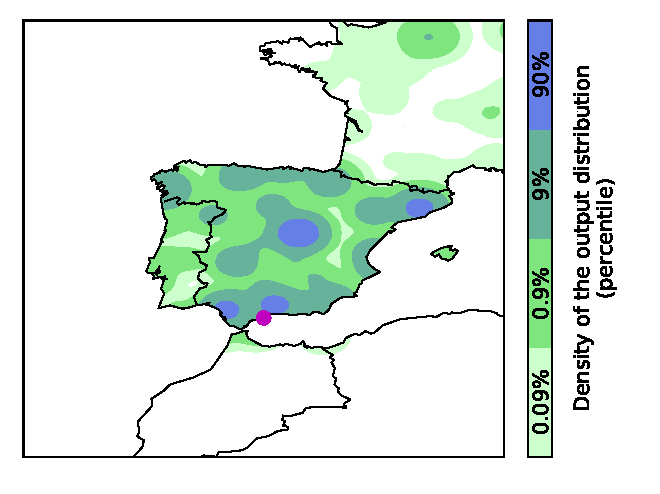
\includegraphics{img/infer/es-vosotros-hablar/0-good-zoom}}
        %\resizebox{0.3\textwidth}{1in}{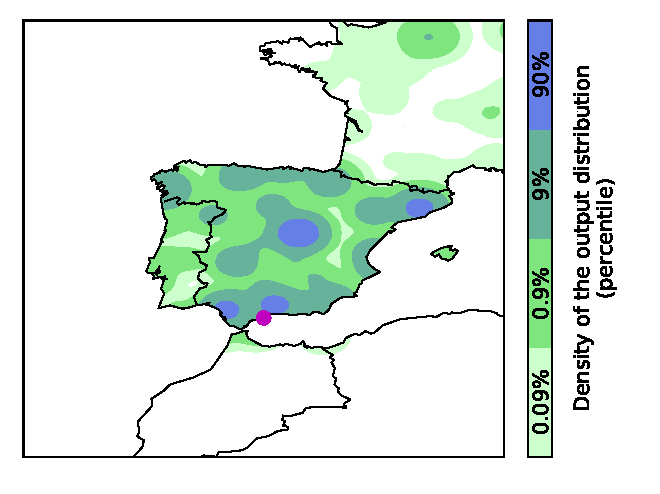
\includegraphics{img/infer/es-vosotros-hablar/0-good-zoom}}
    };
    \node (fvm4) [right=0.8cm of mix.east] {};
    \node (fvm3) [right=1.4cm of mix.east] {};
    \node (fvm) [above=0.1cm of fvm3] { MvMF \\ Output };
    %\node (country2) [above =of fvm.north] {
        %Country Cross Entropy \\ 
        %\resizebox{0.37\textwidth}{!}{\input{img/infer/es-vosotros-hablar/11-lo-bar-country2.pgf}}
    %};
    %\node (country) [output, above=of fvm.north, minimum width=0.32\textwidth, minimum height=2cm,fill=none] {};

    \draw[->] (input) -- (embed);
    \draw[->] (embed) -- (conv);
    \draw[->] (conv) -- (mix);
    %\draw[->] (mix) -- (country);
    \draw[->] (mix) -- (fvm4);
    \draw[->] (conv.225) to[out=270,in=180] (lang);
    \draw[->] (lang) to[out=0,in=270] (mix.315);

\end{tikzpicture}
}
